\documentclass[12pt,a4paper]{article}
\usepackage[utf8]{inputenc}
\usepackage[ngerman]{babel}
\usepackage[T1]{fontenc}
\usepackage{amsmath}
\usepackage{amsfonts}
\usepackage{amssymb}

\usepackage{pgf,tikz}
\usepackage{pgfplots}
\usepackage{csvsimple}
\usepackage{epstopdf}
\usepackage{units}
\usepackage{microtype}
\usepackage{esvect}

\usepackage{hyperref}
\usepackage{graphicx}
\usepackage[left=2cm,right=2cm,top=2cm,bottom=2cm]{geometry}
\setlength{\parindent}{0pt}

\title{Pendel (PEN)}
\author{Kilian Brenner und Carlos Esparza \\ Team 13, Group 6}

\date{2.04.2018}


\pgfplotsset{compat=newest,
    tick label style={font=\small},
    label style={font=\small},
    legend style={font=\footnotesize}
}

%\tikzset{every mark/.append style={scale=0.3}}
\newlength{\plotheight}
\newlength{\plotwidth}
\newlength{\imgheight}
\setlength{\plotwidth}{\textwidth}
\setlength{\plotheight}{11cm}

\newcommand{\e}[1]{\cdot\!10^{#1}}
\renewcommand{\emph}{\textbf}
\newcommand{\C}{\unit{\, ^\circ C}}
\newcommand{\abs}[1]{\left| #1 \right|}
\newcommand{\n}[1]{\mathrm{#1}}
\renewcommand{\vec}[1]{\mathbf{#1}}

\renewcommand{\d}{\mathrm{d}}
\newcommand{\pdiff}[2]{\frac{\partial #1}{\partial #2}}
\DeclareMathOperator{\var}{Var}
\DeclareMathOperator{\cov}{Cov}


\usepackage{mathtools}
%\DeclarePairedDelimiter{\abs}{\lvert}{\rvert}


\begin{document}
\maketitle
\tableofcontents
\newpage

\section{Einleitung}
In diesem Versuch werden die Eigenschaften von verschiedenen Pendeln untersucht. Außerdem erhalten wir eine Methode um die lokale Erdbeschleunigung $g$ experimentell zu bestimmen. 

\section{Verwendete Methoden}
\subsection{Lösungen}
Unter Dissoziation versteht man den Zerfall eines Moleküls in mindestens zwei geladene oder neutrale Bruchstücke. Diese Bruchstücke wechselwirken nun mit den Molekülen des Lösungsmittels (Lösung). Bei einer idealen Lösung überwiegt der Anteil des Lösungsmittels deutlich gegenüber dem zu lösenden Stoff. Allerdings werden meist nicht alle Moleküle des zu lösenden Stoffes aufgespalten. Der Anteil der aufgespaltenen Moleküle zur Gesamtmenge an Molekülen nennt man den Dissoziationsgrad $\alpha$. Zerfällt ein Molekül in z Moleküle und beschreibt N die Anzahl der Moleküle des Lösungsstoffes sowie N' die Anzahl der gelösten Moleküle, so ergibt sich folgender Zusammenhang:

\begin{equation}
N' = N \cdot \alpha \cdot z + N(1-\alpha) \label{eq:N'}
\end{equation}
und somit
\begin{equation}
\alpha = \frac{\frac{N'}{N}-1}{z-1} \label{eq:alpha}
\end{equation}
%
Mithilfe der Anzahl der gelösten Teilchen, kann also der Dissoziationsgrad ermittelt werden. Hierbei wird von der  François Marie Raoult gefundenen Gesetzmäßigkeit, welche den Dampfdruck mit der Teilchenanzahl verknüpft, Gebrauch gemacht. Mithilfe dieser Gesetzmäßigkeit und der Clausius-Clapeyronschen Beziehung ergibt sich unter der in der Aufgabenstellung gegebenen Näherung, dass die Schmelzdruck-Kurven in Abhängigkeit des Drucks von dem Lösungsmittel und der Lösung nahezu parallel sind, und der Vereinfachung, dass die Lösung stark verdünnt ist, folgender Zusammenhang: \footnote{Siehe Aufgabenstellung}

\begin{equation}
\frac{N'}{n} = \frac{\Delta T_G \cdot M_1}{K_{G1} \cdot \unit[1]{kg}}
\end{equation}



\section{Experimentelles Vorgehen}
\subsection{Bestimmung der Schallgeschwindigkeit durch Laufzeitmessung}
Im ersten Versuch soll die Schallgeschwindigkeit durch Laufzeitmessung erfolgen. Hierfür wird wie in Abbildung \ref{fig:versuch1} dargestellt mithilfe eines Oszilloskops die Differenz der Zeit ermittelt, die ein erzeugtes Schallsignal für den Abstand zwischen den zwei Mikrofonen benötigt. Zu beachten bei dem Versuch ist, dass der Abstand der Mikrofone nicht exakt ermittelt werden kann, dafür aber die Abstandsdifferenz. Zudem muss das Schallsignal auf einer Geraden mit den zwei Mikrofonen liegen.\\
Es werden etwa 5-10 Messungen durchgeführt, um einen statistisch guten Wert für die Schallgeschwindigkeit zu erhalten.

\begin{figure}
\begin{center}
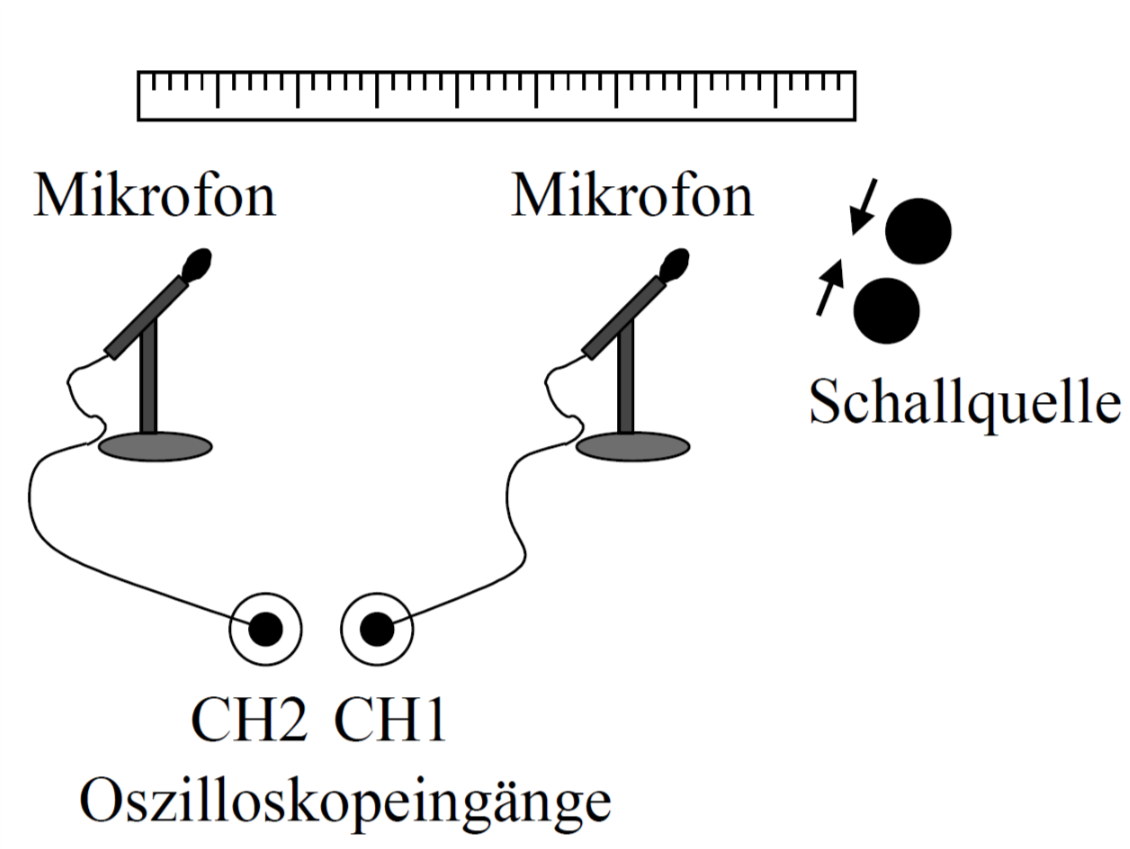
\includegraphics[width=0.5\textwidth]{Bilder/Versuchsaufbau1.png}
\caption{Bestimmung der Schallgeschwindigkeit in Luft durch Laufzeitmessung}
\label{fig:versuch1}
\end{center}
\end{figure}

\subsection{Bestimmung der Schallgeschwindigkeit in Festkörpern}
Im zweiten Versuch soll -- ebenfalls durch Laufzeitmessung -- die Schallgeschwindigkeit in Festkörpern (in diesem Fall in Form von Stäben) bestimmt werden. Hierzu wird (siehe Abb. \ref{fig:versuch2} mit Hilfe eines Piezoelektrischen Körpers, angeschlossen an ein Oszilloskop, der Abstand zwischen zwei Maxima der (longitudinalen) Auslenkungen und damit die Zeit, die ein Schallimpuls für die doppelte Länge des Stabes benötigt. Der Impuls wird durch einen leichten Schlag auf den Stab erzeugt. Auch für diesen Versuch werden mehrere Messreihen, sowie der Abstand von jeweils mehreren Maxima, gemessen.\\
Zudem wird die Schallgeschwindigkeit für drei verschiedene Materialien ermittelt.

\begin{figure}
\begin{center}
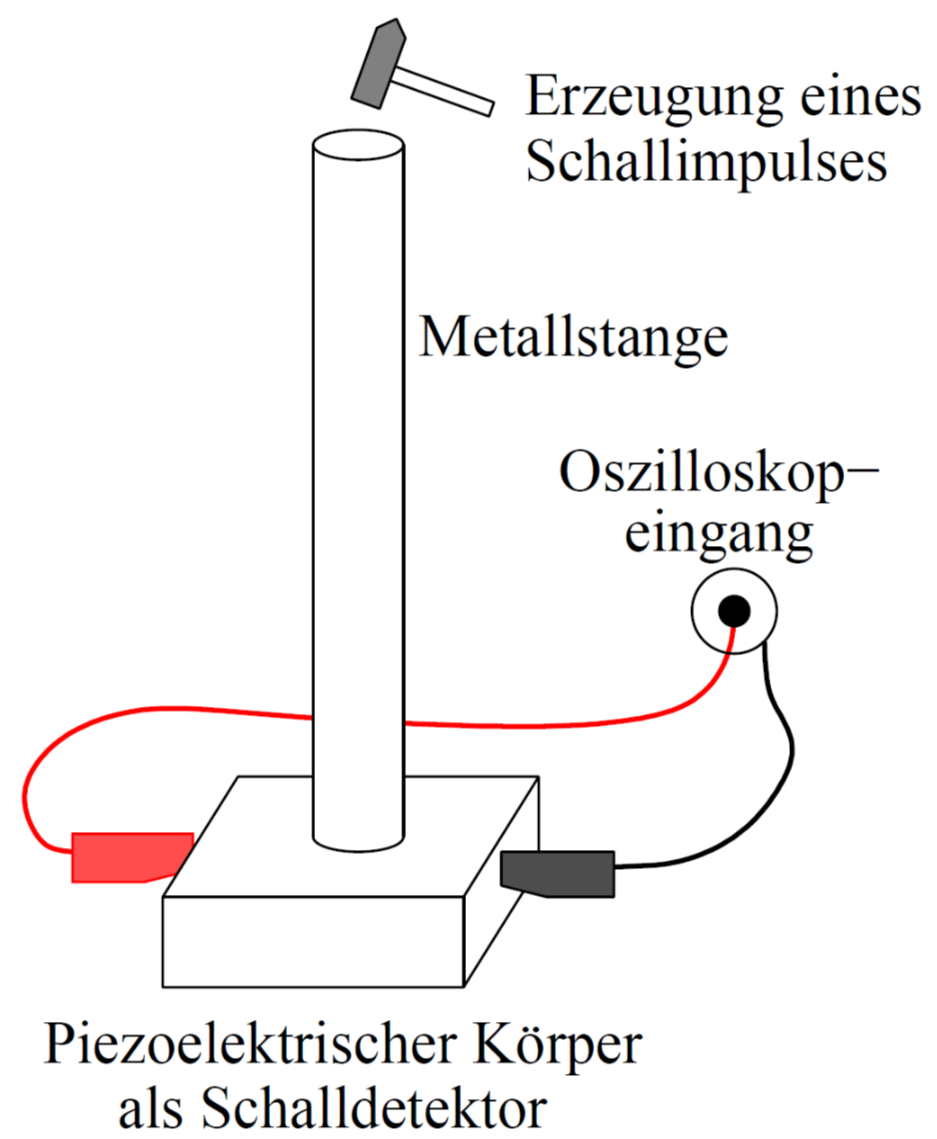
\includegraphics[width=0.3\textwidth]{Bilder/Versuchsaufbau2.png}
\caption{Bestimmung der Schallgeschwindigkeit in Festkörpern durch Laufzeitmessung}
\label{fig:versuch2}
\end{center}
\end{figure}

\subsection{Bestimmung der Schallgeschwindigkeit über stehende Wellen}
In einer Luftsäule wird mit einem Frequenzgenerator eine feste Frequenz angeregt. Mithilfe des in Abbildung \ref{fig:aufgabe3} dargestellten verschiebbaren Stempels wird die Länge der Luftsäule variiert. Es werden die Längen der Luftsäule gemessen, für die eine stehende Welle erzeugt wird, also für die eine Resonanz beobachtet wird. Für drei verschiedene Frequenzen werden möglichst viele Längen der Luftsäule (mit Resonanz) gemessen. Die Messung erfolgt jeweils einmal für eine Verlängerung sowie für eine Verkürzung, sodass zwei Werte für die (theoretisch) gleiche Länge existieren, sodass ein besserer Mittelwert gebildet werden kann. Mithilfe der Gleichung \ref{eq:speedFreq} kann somit die Schallgeschwindigkeit für jeden der ermittelten Längen und der zugehörigen Frequenz berechnet werden.


\begin{figure}
\begin{center}
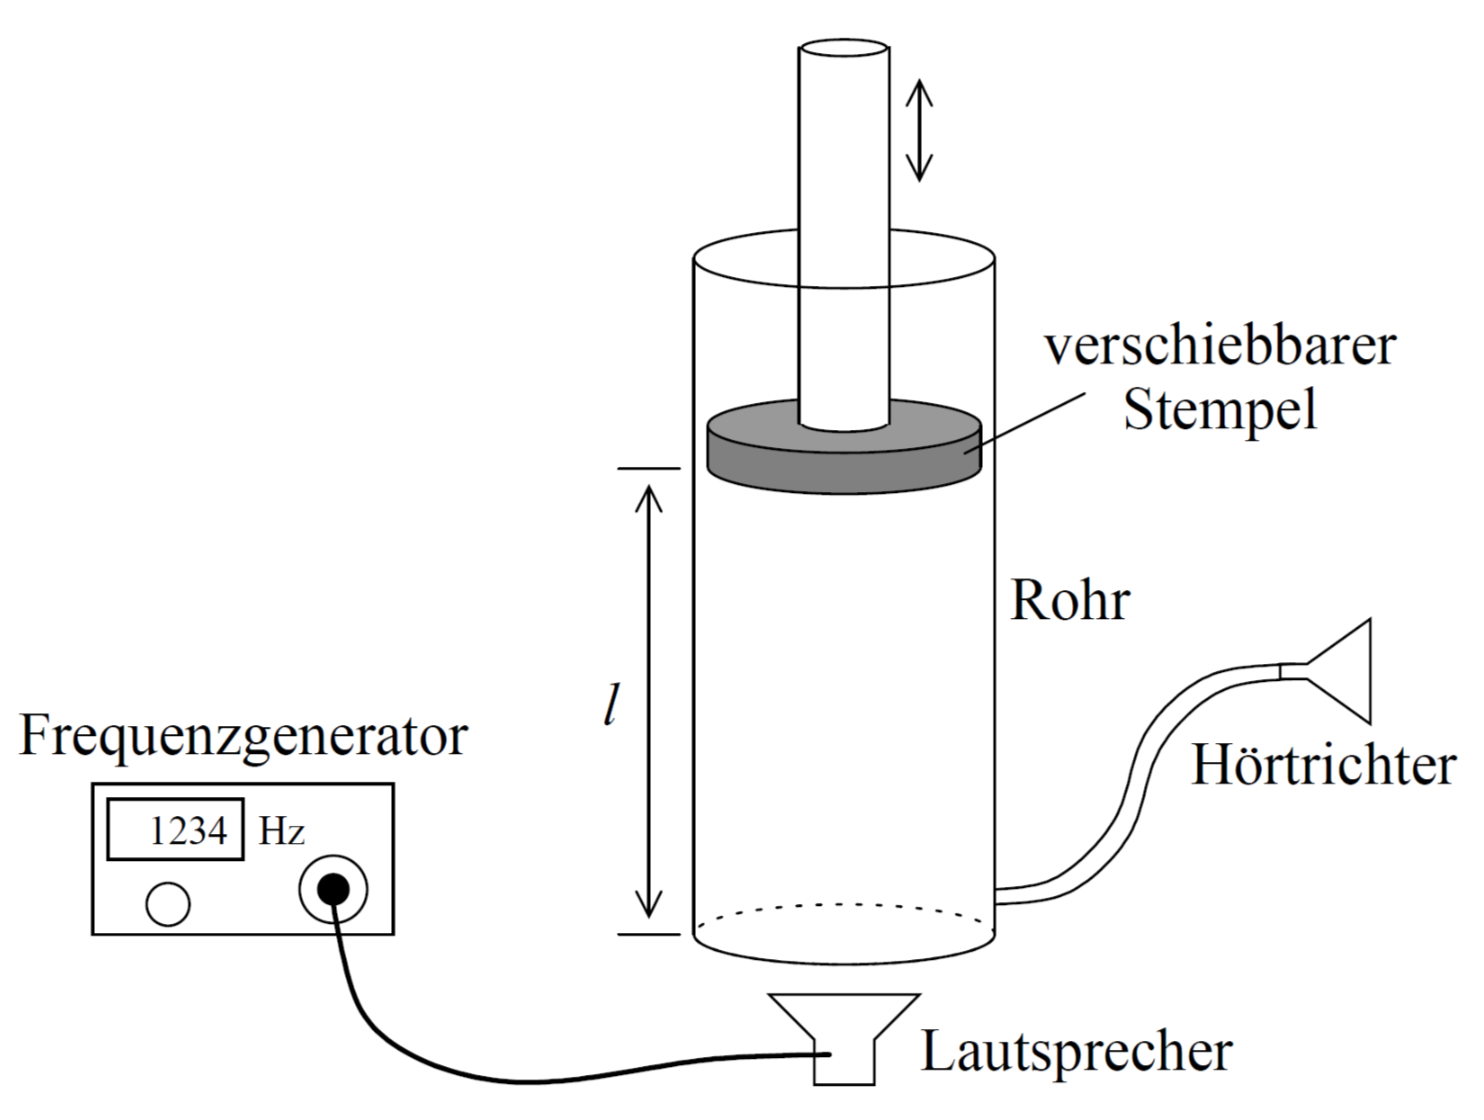
\includegraphics[width=0.3\textwidth]{Bilder/Versuchsaufbau3.png}
\caption{Bestimmung der Schallgeschwindigkeit über stehende Wellen}
\label{fig:versuch3}
\end{center}
\end{figure}




\section{Ergebnisse}
\subsection{Kalibrierung}
\subsection{Kalibrierung der kleinen Scheibe}
Für die kleine Drehscheibe wurden alle $\unit[45]{^\circ}$ die resultierende Kraft bei einem Radius $r = \unit[(18.8 \pm 0.3)]{cm}$ gemessen (siehe Abbildung \ref{fig:kal1}). Mit linearer Regression\footnote{Berechnung durch Origin} bekommen wir eine Steigung von $d = \unit[(221.9 \pm 1.0)]{mN cm}$.\\
Zudem kann die Winkelrichtgröße durch die Steigung ermittelt werden. Durch Formel \ref{eq:wink}:
\begin{equation}
T^2 = \frac{4\pi^2}{d}\cdot (J_0+J_Z)
\end{equation}
Der y-Achsenabschnitt $f = \unit[(0.57 \pm 0.06)]{s^2}$ ergibt sich durch die Regression, und somit ist $J_0$
\begin{align}
J_0 &= f^2\frac{d}{4\pi^2}\\
J_0 &= \unit[18376]{g cm^2}
\end{align}
Somit können wir $d$ berechnen:
\begin{equation*}
d = \frac{4\pi^2}{W} = \unit[(223.3 \pm 1.5)]{mN cm}
\end{equation*}


\begin{figure}
\begin{center}
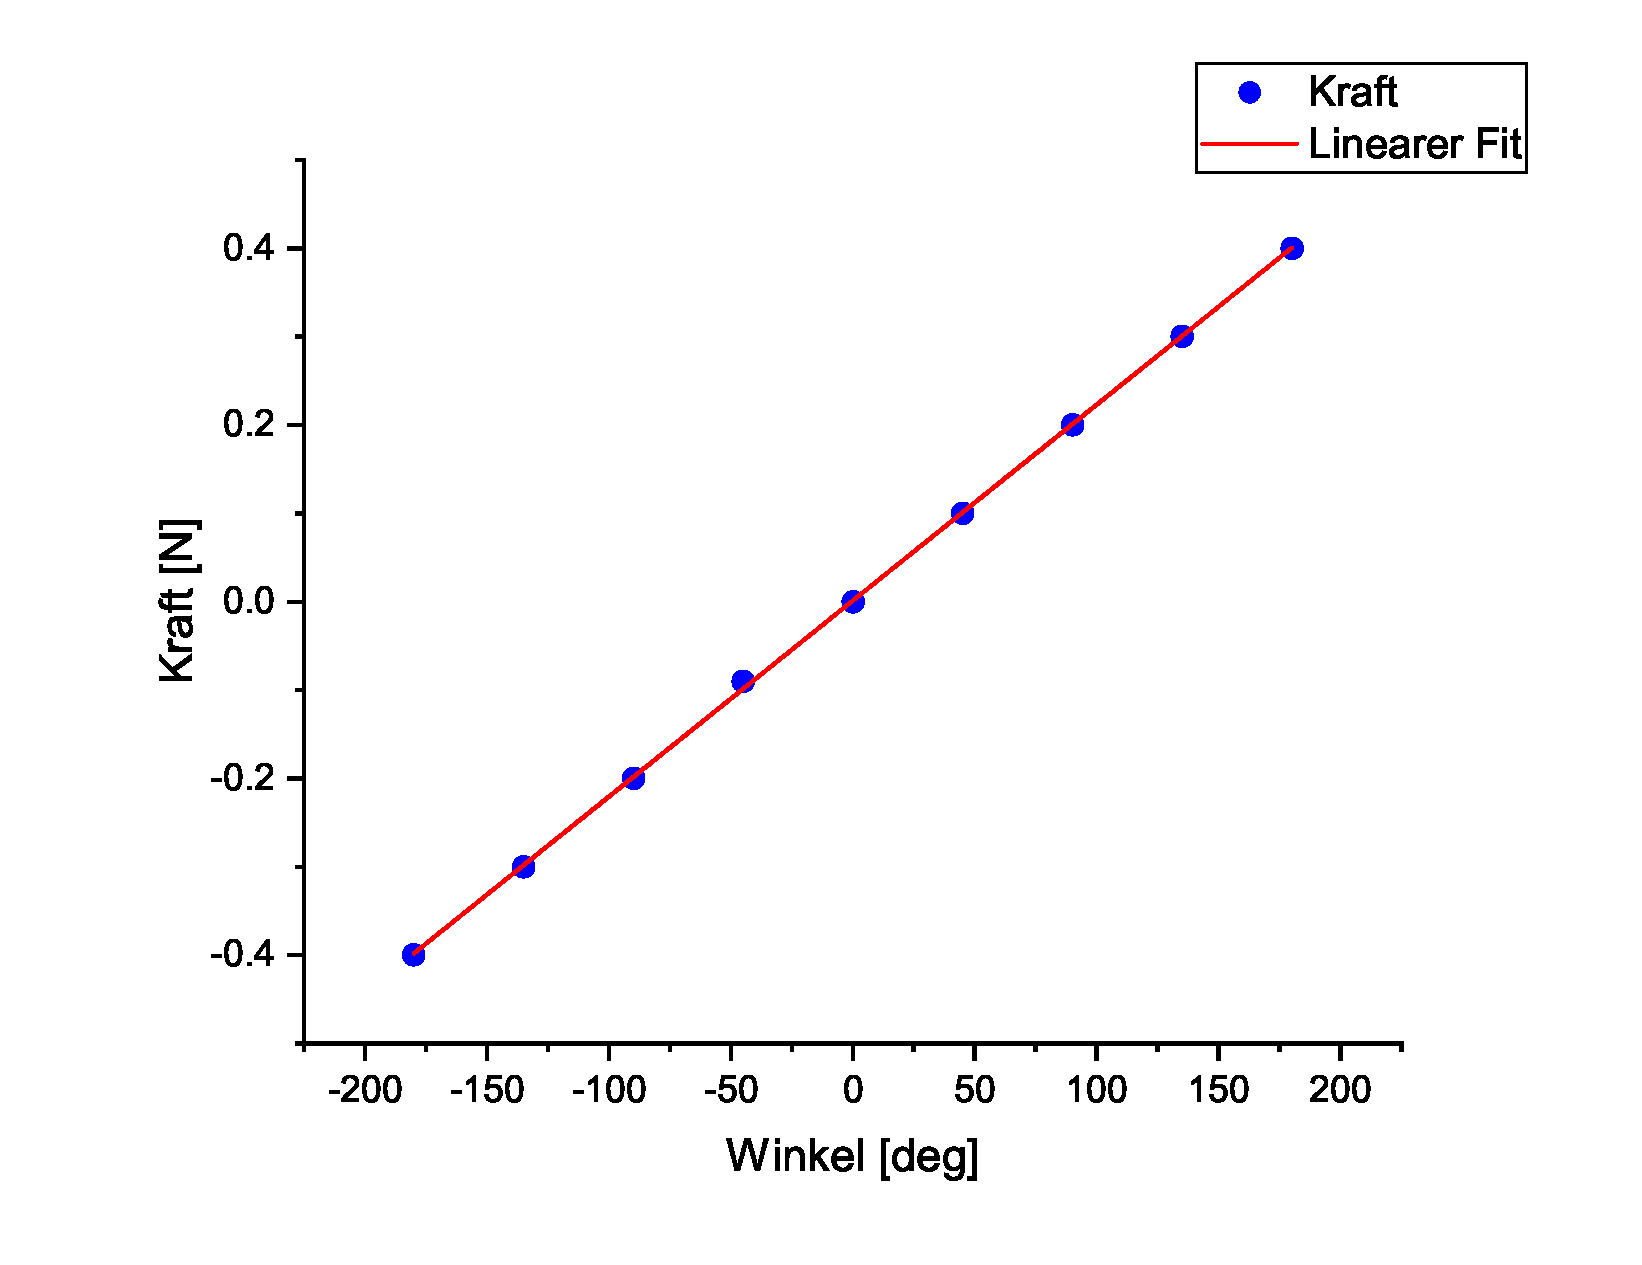
\includegraphics[width=0.7\textwidth]{Bilder/kal1.eps}
\caption{Kalibrierung der kleinen Scheibe}
\label{fig:kal1}
\end{center}
\end{figure}
\subsection{Kalibrierung der großen Scheibe}
Mit der großen Scheibe funktioniert die für die Winkelrichtgröße $D$ genauso wie für die kleine Scheibe. Aus diesem Grund werden hier nur die Werte (inkl. Fehler) angegeben. Es ergibt sich folgender Wert (Daten, siehe Abb. \ref{fig:kal2})
\begin{align*}
D = \unit[(2.17 \pm 0.04)]{N m}
\end{align*}
Die großen Fehlerwerte ergeben sich dadurch, dass die rücktreibende Kraft von der Richtung, in die die Scheibe ausgelenkt wird abhängt (materialbedingt).
\begin{figure}
\begin{center}
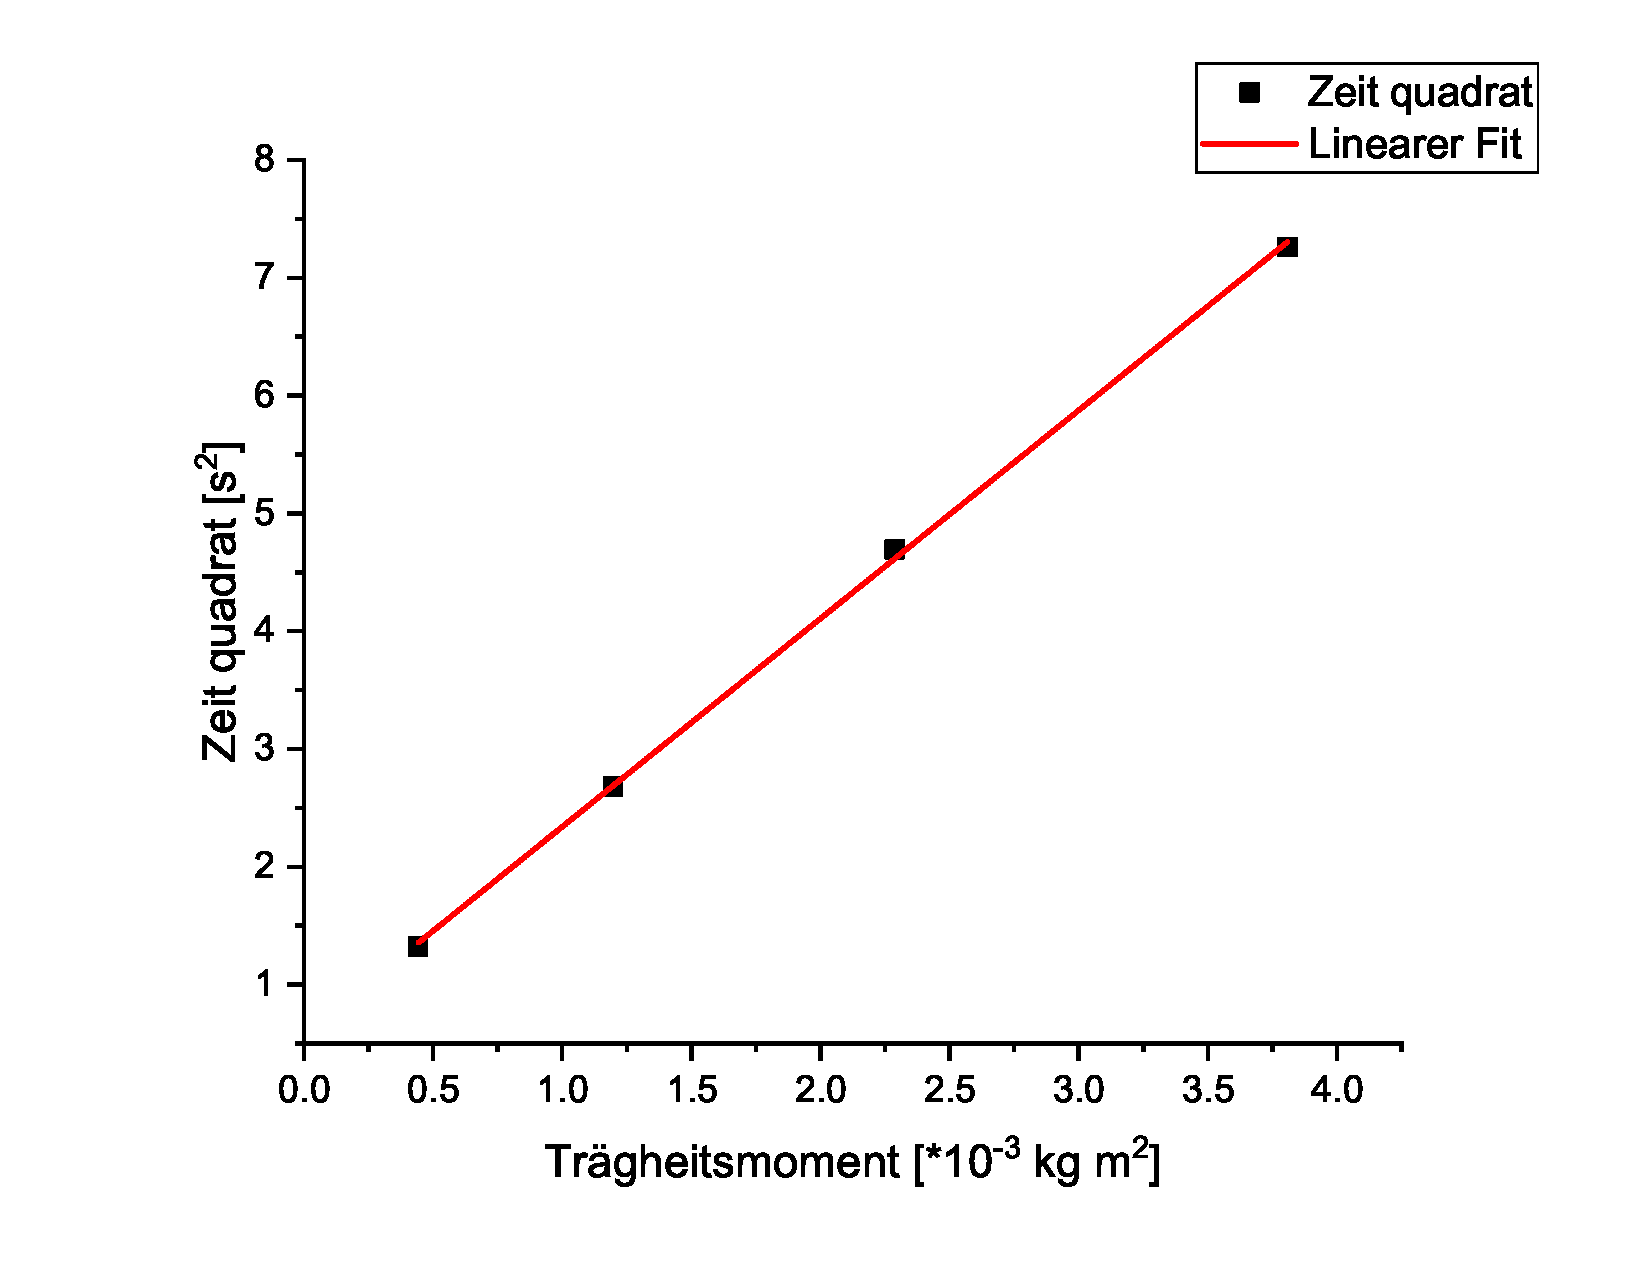
\includegraphics[width=0.7\textwidth]{Bilder/kal2.eps}
\caption{Kalibrierung der großen Scheibe}
\label{fig:kal2}
\end{center}
\end{figure}
Zudem ist das Material sowie die Abmessungen der Scheibe bekannt, also kann der Trägheitmoment berechnet werden:
\begin{equation}
J_0 = \frac{1}{2} m \cdot r^2 = \frac{1}{2} d\cdot r^2 \cdot \rho \pi r^2 = \unit[0.67]{kg m^2}
\end{equation}
Also ergibt sich für die Winkelrichtgröße $D = \unit[(2.27 \pm 0.3)]{N m}$.\\
Dieser relativ große Fehler ergibt sich durch die Ungenauigkeit im Radius, der mit der vierten Potenz in die Rechnung eingeht.







\subsection{Berechnung des Trägheitsmoments durch Approximation des Körpers}

\begin{figure}
\begin{minipage}{.49\textwidth}
    \centering
    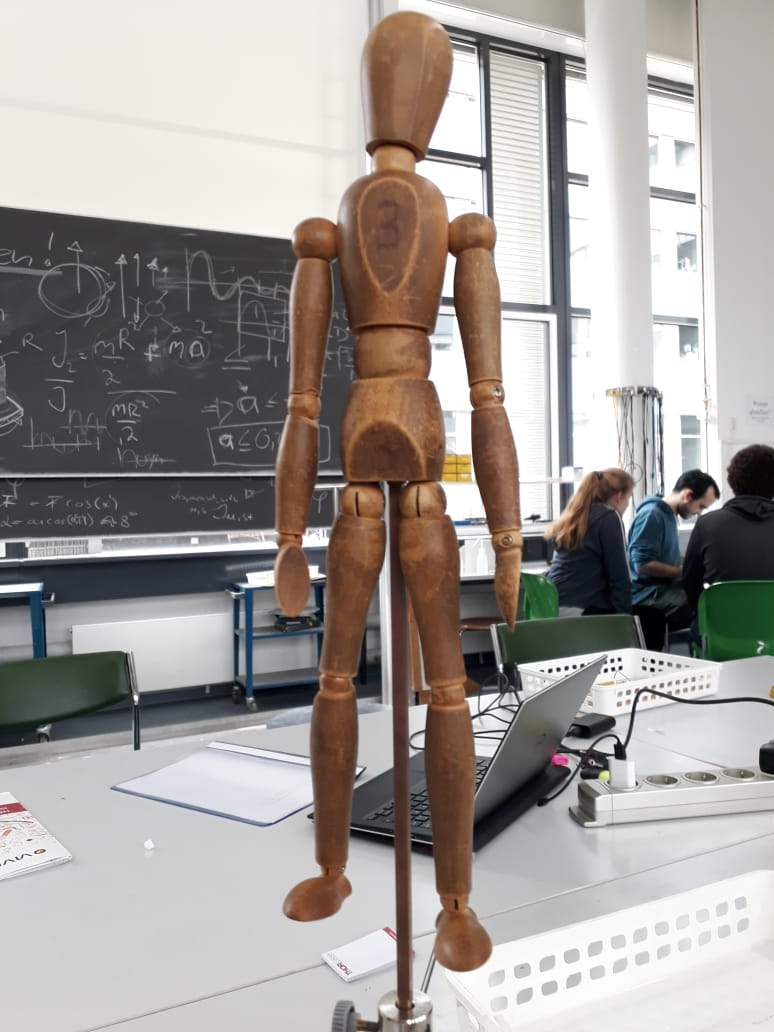
\includegraphics[scale=.28]{./Bilder/figur1.jpeg}
    \caption{Figur 1}
\end{minipage}
\begin{minipage}{.49\textwidth}
    \centering
    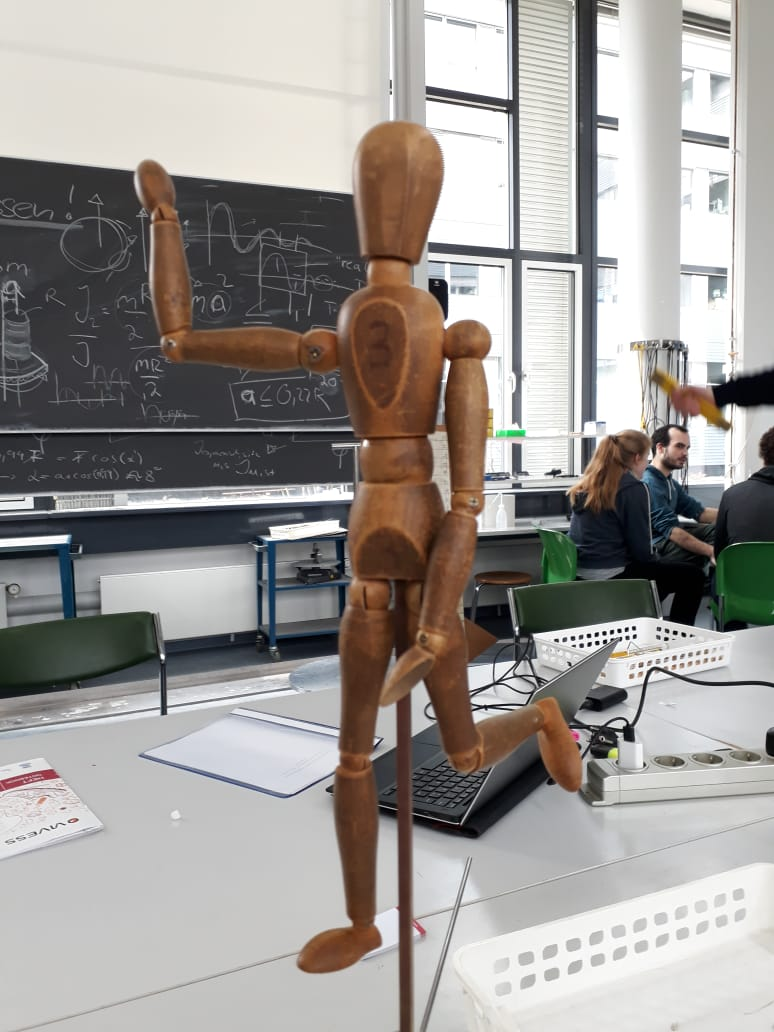
\includegraphics[scale=.28]{./Bilder/figur2.jpeg}
    \caption{Figur 2}
\end{minipage}
\end{figure}


Für Person 1 und Figur 1 errechnen wir ein theoretisches Trägheitsmoment von  $\unit[0.8]{kg\,m^2}$. Für Person 2 und Figur 2 erhalten wir einen Wert von $\unit[1.9]{kg\,m^2}$. 



\section{Diskussion und Zusammenfassung}
In diesem Versuch wurde vor allem der theoretische und tatsächliche Verlauf von Isothermen bei Volumen- und Temperaturänderung behandelt. Wichtige Schlüsse aus diesem Versuch sind die Abweichung von der Theoriekurve (nach Van der Waals), durch die Tatsache, dass sich das Gas unter hohem Druck unterhalb der kritischen Temperatur teilweise verflüssigt und damit den Druck für einen begrenzten Bereich so ausgleicht (genaueres wurde bereits in den verwendeten Methoden behandelt), dass dieser in diesem konstant bleibt. Die Existenz einer solchen kritischen Temperatur und eines dazugehörigen kritischen Drucks (erste und zweite Ableitung sind an diesem Punkt null) ist ebenfalls eine wichtige Erkenntnis.\\
Die Fehlerwerte für die Stoffmenge (siehe Sektion \ref{sec:Stoffmenge}) sind ziemlich klein, was durch die hohe Anzahl von Werten herrührt. Allerdings können diese abweichen, da der Fehlerwert auch von der Art der Extrapolation abhängt (welche nicht vorgegeben ist).\\
Dierecht großen Fehler für die Bestimmung der kritischen Temperatur von $SF_6$ und der Verdampfungsenthalpie ergeben sich durch die nur durch Augenmaß bestimmbaren ''Plateaus'' (Koexistenzbereich von Flüssigkeit und Gas) und die ebenfalls nur durch Augenmaß bestimmbare kritische Temperatur durch den Verlauf des Gas- bzw. Flüssigkeitsvolumens. Selbiges gilt für den kritischen Druck. Zudem sind die durch den menschlichen Faktor erzeugten Fehler (insbesondere die anderer Gruppen) nur schwer abzuschätzen und werden daher eher größer geschätzt. Ein weiterer Faktor sind teilweise abweichende Messungen von der Erwartung, die sich vermutlich unter anderem durch eine schnelle Messung bedingen (insbesondere bei der Messung für ein sich vergrößerndes Volumen), da die Flüssigkeit noch nicht vollständig verdampfen konnte, was den Druck beeinträchtigt.


%\begin{appendix}
%\addcontentsline{toc}{section}{Anhang}
%\section{Fehlerrechnung}
\newcommand{\rg}{R_\mathrm{G}} % zu faul zum Schreiben
\newcommand{\stat}{\Delta} % ich ändere ca. jede Stunde meine Meinung wie ich statistische Fehler bezeichnen soll...

Den statistischen Fehler $\Delta \rg$ des Widerstands bei Schmelztemperatur (destilliertes Wasser) erhalten wir als die Standardabweichung des Mittelwerts aus den 3 Messungen:
%
\begin{align*}
            \rg &= \frac{6.66 + 6.66 + 6.67}{3} \\
        s_{\rg} &= \sqrt{\frac{\left(6.66 - \rg\right)^2 + \left(6.66 - \rg\right)^2 + \left(6.67 - \rg\right)^2}{3 - 1}} \\[1mm]
    \stat \rg  &= \frac{s_{\rg}}{\sqrt{3}} \approx \unit[0.0033]{k\Omega}
\end{align*}
%
Den statistischen Fehler $\stat R_\mathrm{G1}$ für die Salzlösung erhalten wir genauso und er ergibt sich ebenfalls zu $\Delta R_\mathrm{G1} \approx \unit[0.0033]{k\Omega}$.
%Sicherheitshalber berücksichtigen wir auch einen eventuellen systematischen Fehler im Termistor von $\pm \unit[0.005]{k\Omega}$ (halbe Skala).

Den Fehler für die Steigung der linearen Näherung an die Temperatur-Widerstand-Kurve des Termistors erhalten wir allein durch die lineare Regression.
%
Zusammen mit dem Wert $a = \unit[(-3.215 \pm 0.024)]{K\, k\Omega^{-1}}$ für die Steigung der linearen Näherung an die Temperatur berechnen wir die Verschiebung des Schmelzpunktes mithilfe von Gleichung~\ref{eq:DT}. Das Gaußsche Fehlerforpflanzungsgesetz liefert für die statistischen Fehler
%
\begin{align*}
    \stat(\Delta T_\mathrm{G}) &= \sqrt{(R_\mathrm{G} - R_\mathrm{G1})^2 \stat a^2 +
                                                      a^2 (\stat {R_\mathrm{G}}^2 + \stat {R_\mathrm{G1}}^2)} \\
                                              &= \unit[0.020]{K}
\end{align*}
%

Die Unsicherheit bei der Masse des Wassers ergibt sich durch
\[
    \stat(n M_1) = \sqrt{2} \cdot \unit[0.0005]{g} + 2 \cdot \unit[0.0002]{g} \approx \unit[0.0011]{g}
\]
Denn der statistische bzw. systematische Fehler der Waage betragen $\unit[0.0005]{g}$ bzw. $\unit[0.0002]{g}$ und das Gewicht des Wassers wurde indirekt durch wiegen des leeren Reagenzglases und später des vollen Reagenzglases ermittelt.

Der Fehler bei der Stoffmenge des Salzes $N$ ergibt sich aus dem statistischen plus dem systematischen Fehler der Waage, da die Unsicherheit der molaren Masse des Salzes mehrere Größenordnungen kleiner ist%
\footnote{Die molaren Massen von Na, N und O sind in Periodensystemen mit bis zu 4 Nachkommastellen tabelliert, d.\,h.\ der Fehler ist $<0.001\%$}%.

Aufgrund der hohen Genauigkeit der Waage sind diese Fehler im Folgenden jedoch irrelevant: 
%Vergleicht man den Beitrag von $\stat (\Delta T_\mathrm{G})$ und $\stat(n M_1)$ in Gleichung~\ref{eq:N'} sieht man:
%
%\begin{align*}
%    \frac{\partial N'}{\partial \Delta T_\mathrm{G}} \stat(\Delta T_\mathrm{G}) &= \frac{n M_1}{K_\mathrm{G1}}
%\end{align*}
%
In Gleichung~\ref{eq:N'} hat $\Delta T_\mathrm{G}$ einen relativen Fehler%
\footnote{Da es sich bei bei Gleichungen~\ref{eq:N'} und \ref{eq:alpha} grundsätzlich nur um Multiplikationen und Divisionen handelt kann man einfach die relativen Fehler vergleichen.}
von ca.\ $2\%$, $n M_1$ jedoch nur einen von ca.\ $0.005\%$. Folglich hat auch $N'$ in Gleichung~\ref{eq:alpha} einen relative Fehler von $2\%$ somit also deutlich mehr als $N$ mit nur ca.\ $0.1\%$. Die Fehler ergeben sich somit als
%
\begin{align*}
        \stat N' &= \frac{n M_1}{\unit[1]{kg}} \stat(\Delta K_\mathrm{G}) \approx \unit[0.22\cdot\! 10^{-3}]{mol} \\
    \stat \alpha &= \frac{\stat N'}{N (z-1)} \approx 0.016
\end{align*}
%







%\end{appendix}


\end{document}
